\section{System}
\label{sec:sys}

\begin{figure}[t!]
\begin{center}
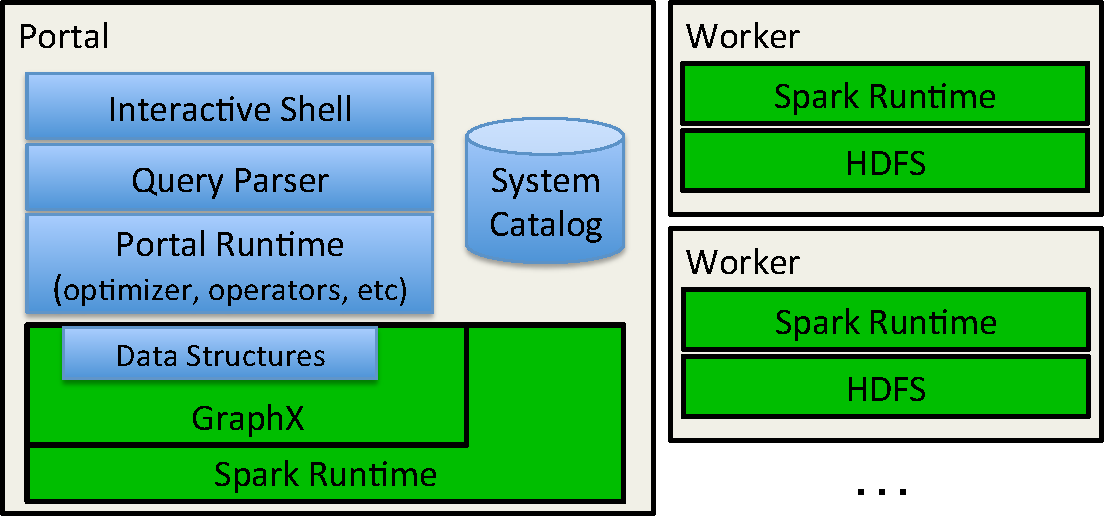
\includegraphics[height=1.4in]{figs/architecture.pdf}
\caption{\ql system architecture.}
\label{fig:arch}
\end{center}
\end{figure}

Our \ql system implementation builds on GraphX, an Apache Spark
library, as depicted in Figure~\ref{fig:arch}.  Green boxes indicate
built-in components, while blue are those we added for \ql.  We
selected Apache Spark because it is a popular open-source system, and
because of its in-memory processing approach.  All language operators
are available through the public API of the \ql library, and may be
used like any other library in an Apache Spark application.  We are
currently working on the query language and query optimization
components on the system.  Since the focus of this paper is the
evolving graph model and algebra, as well as the efficiency of various
physical representations of this model for carrying out these
algebraic operations, we leave the description of the query aspects of
\ql for a subsequent paper.

\subsection{Physical Represenatations}
\label{sec:sys:datastructs}

We considered four in-memory \tg representations that differ in
compactness, but also, perhaps more importantly, in the kind of
locality they prioritize. With {\em structural locality}, neighboring
vertices of the same snapshot are laid out together, while with {\em
  temporal locality}, consecutive states of the same vertex are laid
out together.  VertexEdgeGraph (VE) is a direct translation of the
vertex-edge relations model and the most compact representation.
SnapshotGraph (SG), a representation in which each representative
graph is stored explicitly, naturally preserves structural locality,
but temporal locality is lost. OneGraph (OG) stores all vertices and
edges of an evolving graph once, in a single data structure.  This
representation emphasizes temporal locality, while also preserving
structural locality.  HybridGraph (HG) trades compactness for better
structural locality, by aggregating together several consecutive RGs,
and computing a OneGraph for each graph cluster.  We can convert from
one representation to any other at small or no cost, so it is useful
to think of them as access methods in the context of individual
operations.

{\bf VertexEdgeGraph (VE).} VEGraph is a direct translation of the
vertex-edge TGraph data model: one RDD contains all the vertices and
another all the edges.  This representation supports all the algebraic
operations on TGraph but cannot support analytics.  As we will show,
due to compactness this physical representation is the most efficient
for many operations.

{\bf SnapshotGraph (SG).} The simplest way to represent an evolving
graph is by representing each representative graph individually, a
direct translation of our RG logical data model.  We call this data
structure SnapshotGraph, or SG for short. An example of an SG is
depicted in Figure~\ref{fig:tg_rg}.  SG is a collection of graphs,
where vertices and edges store the attribute values for the specific
time interval.  This representation supports all the operations
defined for TGraphs, with the exception of
\insql{select}. \insql{select} is only supported in cases without a
predicate on the time period.  To construct SG from V and E we
iteratively select from V and E for each time period.

While the SG representation is simple, it is not compact, considering
that in many real-world evolving graphs there is a 80\% or larger
similarity between consecutive
snapshots~\cite{DBLP:journals/tos/MiaoHLWYZPCC15}.  In a distributed
architecture, however, this data structure provides some benefits as
operations on it can be easily parallelized, by assigning different
RGs to different workers, or by partitioning an RG across workers.

\begin{figure}[t!]
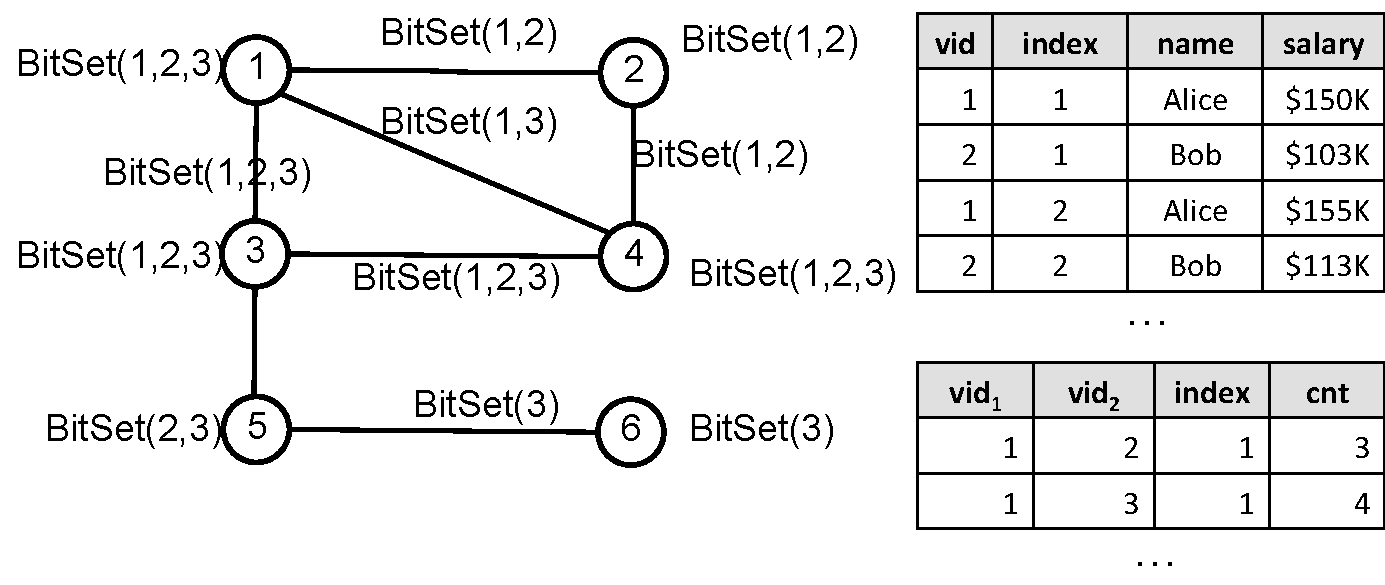
\includegraphics[width=3.2in]{figs/ogc.pdf}
\caption{OG representation of T1 from~\ref{fig:tg_t1}.}
\label{fig:ogc}
\end{figure}

{\bf OneGraph (OG).}  The most topologically compact representation is
to store each vertex {\em and} each edge only once for the whole
evolving graph, by taking a union of the vertex and edge sets.  The
OneGraph data structure, or OG for short, depicted in
Figure~\ref{fig:ogc} uses this representation in our system.  The
drawback is that OG is much denser than individual graphs of SG.  OG
represents only the graph structure, which is sufficient for many
graph analytics.  As a result, this data structure only supports
operations on topology: analytics and aggregation/union/intersection
for graphs with no attributes or when attributes are not relevant for
analysis.  To construct OG vertices and edges from V and E relations
each are grouped by key and mapped to bitsets to represent
presence/absence in each time period of \tg.  In general, because OG
represents topology only, many fewer periods need be represented and
computed than there are RGs in \tg.  The reduction depends on the rate
and nature of the graph evolution.

{\bf HybridGraph (HG).} As an intermediate representation between SG
and OG, we implement the HybridGraph (HG) data structure.  HG is a
series of OGs, with each OG representing some number of temporally
adjacent RGs.  In our current implementation each OG in the sequence
corresponds to the same number of temporally adjacent graphs.  This is
the simplest clustering method, yet, as we will see in
Section~\ref{sec:exp}, it already improves performance compared to OG.
However, we also observed that placing the same number of graphs into
each cluster often results in unbalanced cluster sizes.  This is
because networks commonly exhibit strong temporal skew, with later RGs
being significantly larger than earlier ones.  Consequently, we are
currently working on more sophisticated clustering approaches that
would lead to better balance, and ultimately to better performance.
Like OG, this representation only supports topology-based analyses and
need not represent every RG but only structure-based changes.

\subsection{Maintenance Operations}
\label{sec:sys:maint}

\begin{figure}
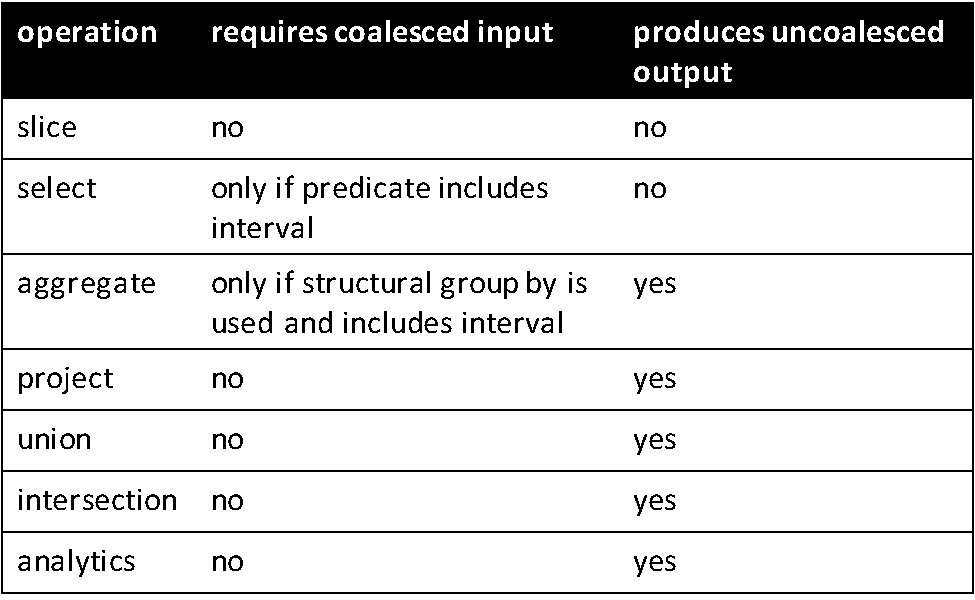
\includegraphics[width=3.2in]{figs/coalesce.pdf}
\caption{Coalesce analysis.}
\label{fig:coalesce}
\end{figure}

{\bf Coalescing.}  The TGraph logical data model is temporally
coalesced.  Portal supports both eager and lazy coalescing, with lazy
being the default behavior.  The final output is always coalesced.
For most operations, correctness of the operation does not depend on
whether the data is or is not coalesced in advance.  For example,
\insql{slice} operation is agnostic to whether a TGraph is coalesced
and does not change the coalesce state.  \insql{select} operation, on
the other hand, is only correct if the data is coalesced when the
selection predicate references the time period.  We analyzed all
operations for their coalescing requirements and whether the operation
causes uncoalescing~\ref{fig:coalesce}.  Additionally, when the
operations are performed on multiple graphs (such as in SG and HG),
the result must also be coalesced to be correct, regardless of the
operation.

There are several different implementations possible for
implementation of the coalesce operation
(see~\cite{DBLP:conf/vldb/BohlenSS96} for detailed analysis in a
non-graph domain).  We use a partitioning method, where the relation
(V or E) is grouped by key, and within each group the tuples are
sorted and folded to produce the longest valid periods.  This approach
involves shuffling between partitions, one of the most computationally
expensive aspects of distributed systems, and thus lazy coalescing is
preferred in the general case.  As with duplicate elimintation, if the
coalesced output is expected to be significantly reduced in size, such
as after a project operation on a high volatility attribute,
performing coalesce eagerly before a consuming operation, especially
analytics, can be advantageous.  We are investigating this further now
for query optimization purposes.

{\bf Foreign key constraint.}  The vertex-edge data model includes a
foreign key constraint from edges to vertices.  This constraint is
naturally maintained by most operations while performing operations on
V and E independently.  For \insql{select} and \insql{aggregate}
additional steps are required to insure correctness.  We modify E
tuples to enforce the foreign key constraint by joining on V, using
either a broadcast or hash join depending on the size of V.  Each edge
period is then modified to be the overlap of the periods of source and
destination vertices and the original edge period.  Because this step
is computationally expensive, it is only taken when necessary: when
\insql{select} has a predicate on V and when \insql{aggregate} has a
higher level of quantification for V than for E.
